% Literature review: published OPA1 perturbation, imaging and rescue evidence.
% Primary source detail, image crops and licenses: docs/opa1-literature.md and provenance JSON.

\begin{frame}[label={sec:org0000009}]{OPA1 links genes to mitochondrial shape}
\begin{itemize}
\item OPA1 is a dynamin-related GTPase in the mitochondrial inner membrane.
\item It supports inner-membrane fusion and mitochondrial network organization.
\item OPA1 depletion produces fragmented mitochondrial networks.
\end{itemize}
\bigskip
\textbf{A genetic example with a recognizable imaging phenotype.}
\par\bigskip
{\scriptsize\href{https://doi.org/10.1083/jcb.200704112}{Griparic et al., JCB (2007)}; \href{https://doi.org/10.1083/jcb.200704110}{Song et al., JCB (2007)}}
\end{frame}

\begin{frame}[label={sec:org000000a}]{OPA1 depletion fragments mitochondria}
\begin{columns}[c,onlytextwidth]
\begin{column}{0.48\textwidth}
\centering\textbf{Control siRNA}\par\medskip
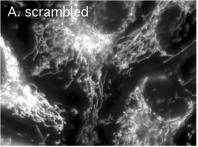
\includegraphics[width=0.88\linewidth,height=0.54\textheight,keepaspectratio]{assets/opa1-literature/control-siRNA-panel-A.png}
\end{column}
\begin{column}{0.48\textwidth}
\centering\textbf{OPA1 siRNA}\par\medskip
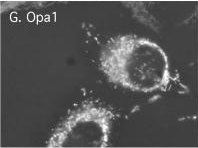
\includegraphics[width=0.88\linewidth,height=0.54\textheight,keepaspectratio]{assets/opa1-literature/OPA1-siRNA-panel-G.png}
\end{column}
\end{columns}
\medskip
\centering {\small HeLa cells; MitoTracker; OPA1 depletion for 48 hours.}\par\medskip
{\scriptsize\href{https://doi.org/10.1083/jcb.200704112}{Griparic et al., JCB (2007), Fig. 3A,G}; cropped panels, \href{https://creativecommons.org/licenses/by-nc-sa/4.0/}{CC BY-NC-SA 4.0}}
\end{frame}

\begin{frame}[label={sec:org000000b}]{A phenotype that can be scored}
\begin{columns}[T,onlytextwidth]
\begin{column}{0.48\textwidth}
\textbf{Read the network}
\begin{itemize}
\item Tubular mitochondria form elongated, connected structures.
\item Fragmented mitochondria appear as short, separate objects.
\end{itemize}
\end{column}
\begin{column}{0.48\textwidth}
\centering
{\Huge\bfseries 99\%}\par\medskip
Cells with fragmented mitochondria after OPA1 siRNA.
\end{column}
\end{columns}
\par\bigskip
{\scriptsize\href{https://pmc.ncbi.nlm.nih.gov/articles/PMC2064541/}{Griparic et al., JCB (2007), Results and Fig. 3}}
\end{frame}

\begin{frame}[label={sec:org000000c}]{Re-expression connects OPA1 to fusion}
\begin{itemize}
\item OPA1-null mouse fibroblasts have fragmented mitochondria.
\item Fusion-active OPA1 splice forms restore tubular networks.
\item A cell-hybrid assay measures recovery of mitochondrial fusion.
\end{itemize}
\bigskip
\textbf{Depletion, imaging and rescue build the biological explanation.}
\par\bigskip
{\scriptsize\href{https://doi.org/10.1083/jcb.200704110}{Song et al., JCB (2007), Fig. 1C,D}}
\end{frame}

\begin{frame}[label={sec:org000000d}]{Workflow 1: follow a gene from the papers to JUMP}
\textbf{Search: OPA1}\par\bigskip
\begin{tabular}{@{}l l@{}}
\textbf{Perturbation} & \textbf{Available in JUMP} \\[7pt]
CRISPR knockout & Yes \\
ORF overexpression & Yes
\end{tabular}
\bigskip
\begin{itemize}
\item Follow the gene to its perturbation identifiers.
\item Open the published feature, match and image tables.
\item Use the Hub's worked examples to follow each step.
\end{itemize}
\par\smallskip
{\scriptsize\href{https://broadinstitute.github.io/jump_hub/reference/00_gene_index.html}{JUMP Hub gene availability}; \href{https://zenodo.org/records/16883068}{coverage reference}}
\end{frame}

\TutorialAvailabilitySlide
\TutorialDefinitionsSlide
\TutorialFiltersSlide
\TutorialExportSlide

\begin{frame}[label={sec:org0000010}]{Workflow 2: read the returned phenotype}
\begin{enumerate}
\item Read overall activity and the changing features.
\item Compare CRISPR and overexpression.
\item Follow similar profiles to their annotations and images.
\item Bring in controls from the same source and plates.
\end{enumerate}
\bigskip
\textbf{Worked examples: SLC2A2 for the tables; MYT1 for the image gallery.}
\end{frame}

\TutorialRowsSlide
\TutorialActivitySlide
\TutorialFeaturesSlide
\TutorialOrfSlide
\TutorialMatchesSlide
\TutorialGallerySlide
\TutorialControlsSlide

\begin{frame}[label={sec:org000000f}]{Bring the workflow together with an agent}
\begin{block}{Start with the papers}
Find primary studies linking OPA1 depletion to mitochondrial fragmentation. Show the control and perturbed images, then summarize the genetic perturbation, imaging readout and main finding.
\end{block}
\medskip
\textbf{Follow the gene into JUMP:}\par
``Find OPA1 in the Hub. Link the availability, feature, match and image resources, then explain how to read each view using the tutorial examples.''
\par\bigskip
\textbf{Output:} a cited biological summary and a linked route through the data.
\end{frame}
